\documentclass[a4paper,10pt]{article}
\usepackage[utf8]{inputenc}
\usepackage{polski}
\usepackage{graphicx}
\usepackage{listings}
\usepackage[usenames,dvipsnames]{color}
\addtolength{\hoffset}{-1cm}
\addtolength{\voffset}{-2cm}
\addtolength{\textwidth}{2cm}
\addtolength{\textheight}{3cm}
\usepackage{setspace}
\usepackage{indentfirst}
\usepackage{graphicx}
\lstset{
    language=Matlab,
    basicstyle=\scriptsize,
    aboveskip={1.5\baselineskip},
    columns=fixed,
    showstringspaces=false,
    extendedchars=true,
    breaklines=true,
    tabsize=4,
    prebreak = \raisebox{0ex}[0ex][0ex]{\ensuremath{\hookleftarrow}},
    frame=single,
    showtabs=false,
    showspaces=false,
    showstringspaces=false,
    identifierstyle=\ttfamily,
    keywordstyle=\color[rgb]{0,0,1},
    commentstyle=\color[rgb]{0.133,0.545,0.133},
    stringstyle=\color[rgb]{0.627,0.126,0.941},
    numbers=left,
    numberstyle=\tiny,
    stepnumber=1,
    numbersep=5pt,
    captionpos=b,
    escapeinside={\%*}{*)}
}

\def\figurename{Rys.}
\def\lstlistingname{Fun.}

\title{Informatyczne Systemy Sterowania \\ \large Ćwiczenie 3: Regulacja dwu- i trójpołożeniowa}

\author{Adam Jordanek 168139, Tomasz Klimek 168092}

\begin{document}
\maketitle

\section{Wstęp}\label{sec:wstęp}
\subsection{Cel ćwiczenia}
Celem tego ćwiczenia jest symulacja działania systemu regulacji z przekaźnikami dwu- i trójpołożeniowymi. Ćwiczenie umożliwić zapoznanie się z nieliniowymi algorytmami sterowania (przełącznikami dwu- i trójpołożeniowymi) oraz zapoznanie się ze środowiskiem Simulink oraz Matlab w zakresie nieliniowych algorytmów sterowania.
%Czy to jest dobrze?

\subsection{Plan badań} 
\begin{enumerate}
	\item Symulacja systemu regulacji. Dobór parametrów regulatora. \newline
	%czy to jest poprawne gramatycznie? :P
	 \small {W trakcie realizacji zadania należy zasymulować działanie systemu regulacji pracującego z regulatorem oraz należy zbadać wpływ wartości parametrów przekaźników na przebieg błędu regulacji}
	\begin{enumerate}
		\item Regulator dwupołożeniowy bez histerezy.
		\item Regulator dwupołożeniowy z histerezą.
		\item Regulator trójpołożeniowy bez histerezy.
		\item Regulator trójpołożeniowy z histerezą.
 	\end{enumerate}
	\item Zastosowanie członów korekcyjnych.
	\begin{enumerate}
		\item Modyfikacja systemów z zadania 1 o korekcję w postaci członu liniowego o transmitancji: 
			\begin{equation} \label{eqn:czlonKorekcyjny}
				K_{k}(s) = {k_{k}} \over {T_{k}s+1}
			\end{equation}
		\item Doświadczalny dobor parametrów członu korekcyjnego.
	\end{enumerate}
\end{enumerate}

\subsection{Podział zadań. (?)} 
\begin{enumerate}
		\item Jordanek Adam
		\begin{enumerate}
			\item Podpunkt jakiś
			\item Inny podpunkt
 		\end{enumerate}
		\item Klimek Tomasz
		\begin{enumerate}
			\item Zbudowanie modeli
			\item Coś
 		\end{enumerate}
\end{enumerate}

\newpage
\section{Realizacja planu i wyniki}
%--------------------------------------------------------------------------------------------------------------------------------
%ZADANIE 1
%--------------------------------------------------------------------------------------------------------------------------------
\subsection{Symulacja systemu regulacji. Dobór parametrów regulatora.}\label{sec:zad1}

\subsubsection{Regulator dwupołożeniowy bez histerezy}\label{sec:r2bh}%----------------------------------------------------------
System regulacji będziemy symulować przy użyciu programu Simulink będącego częścią pakietu M\small ATLAB. \\
\normalsize Schemat systemu służącego nam do symulacji przedstawiony został na poniższym rysunku.

\begin{figure}[!h]
    \centering
	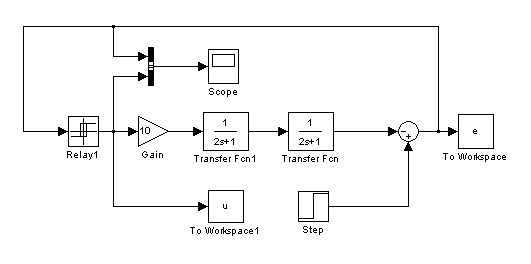
\includegraphics[width=120mm]{CW3-schemat-2.png}
	\caption{Schemat symulacji regulatora dwupołożeniowego.}
    \label{fig:Rysunek}
\end{figure}

Aby zasymulować regulator dwupołożeniowy bez histerezy musimy ustawić parametry 'On' i 'Off' obiektu 'Relay1' na wartość 0. \\
Za przeprowadzenie testu odpowiedzialna jest poniższa funkcja.

\begin{lstlisting}[caption=Funkcja testująca regulator dwupoziomowy bez histerezy.]
function testDwupoziomowy1(step, flag)
load_system('dwupoziomowy.mdl');
hold on;

set_param('dwupoziomowy/Relay1', 'On_switch_value', num2str(0));
set_param('dwupoziomowy/Relay1', 'Off_switch_value', num2str(0));

sim('dwupoziomowy.mdl');
figure(1);
uwy= u.signals.values;    
plot(tout, uwy, '-k');

figure(2);

if flag
    hold on;
    plot([0 20], [0 0], '-r');
end

ewy= e.signals.values;    
plot(tout, ewy, '-k');
end
\end{lstlisting}

Po wywołaniu tej funkcji otrzymaliśmy poniższe wykresy.

\begin{figure}[!h]
    \centering
	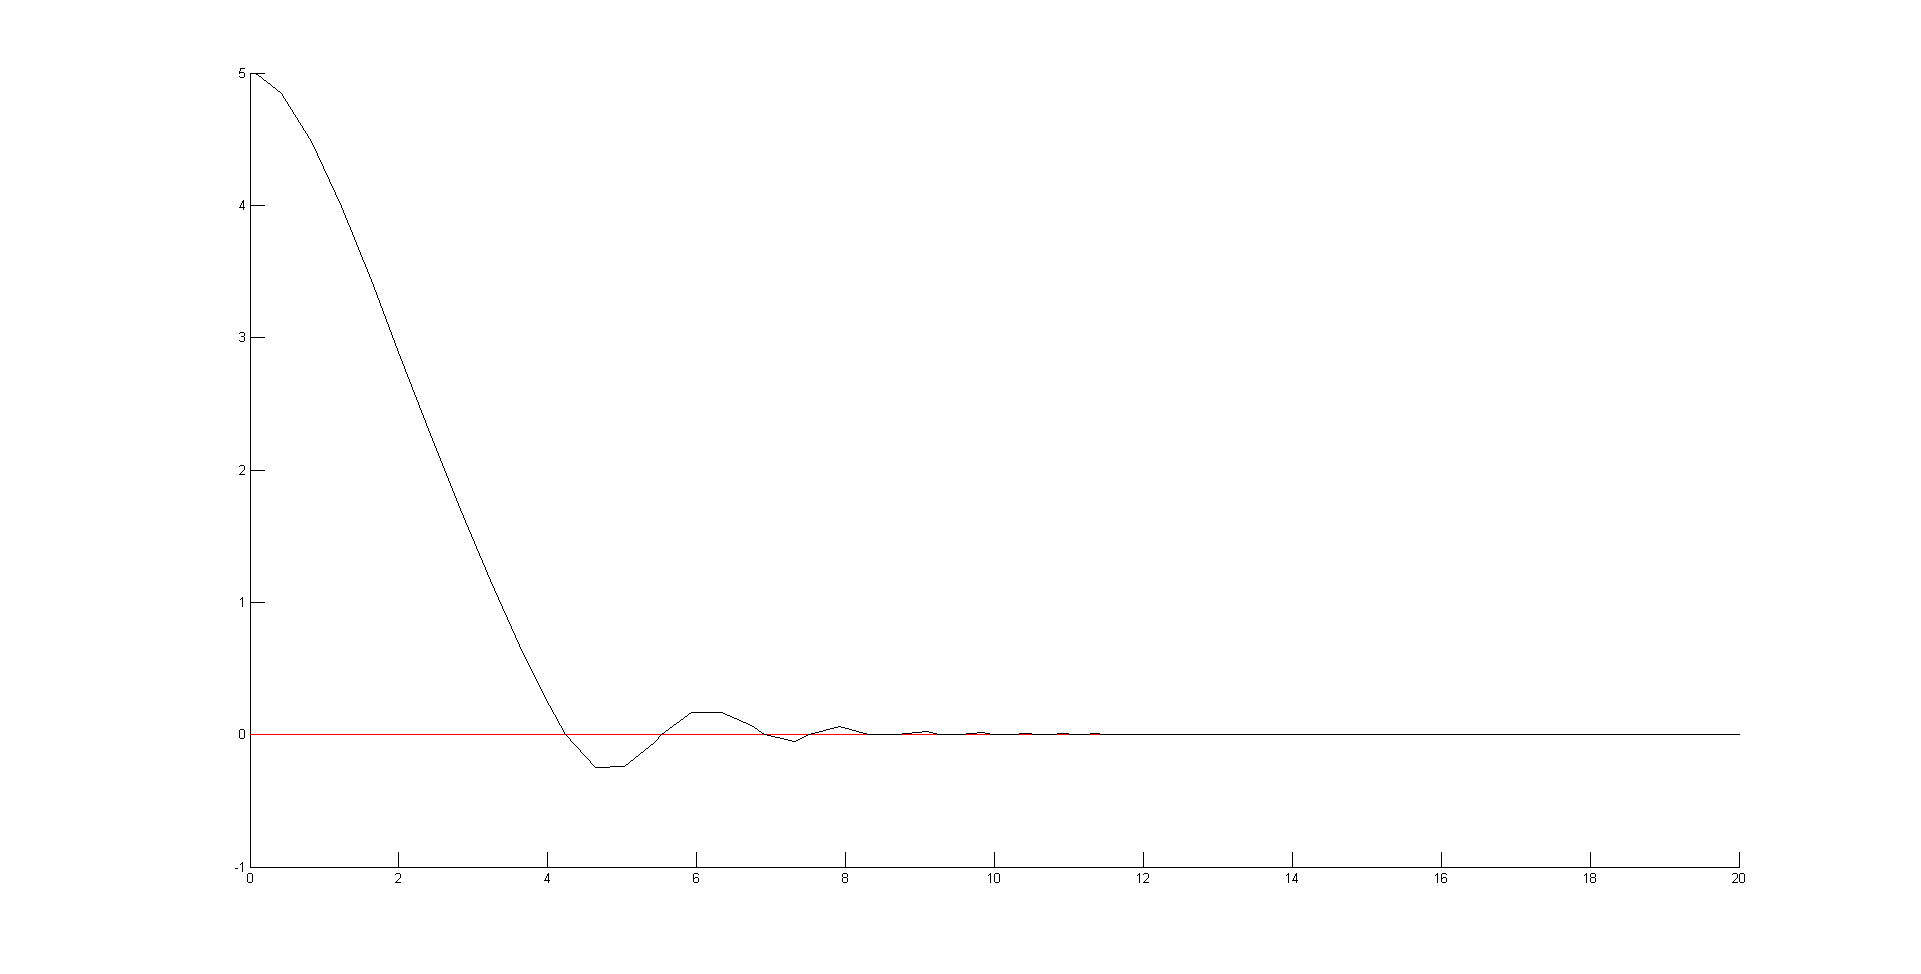
\includegraphics[width=120mm]{CW3-dwupolozeniowy-e-a0.png}
	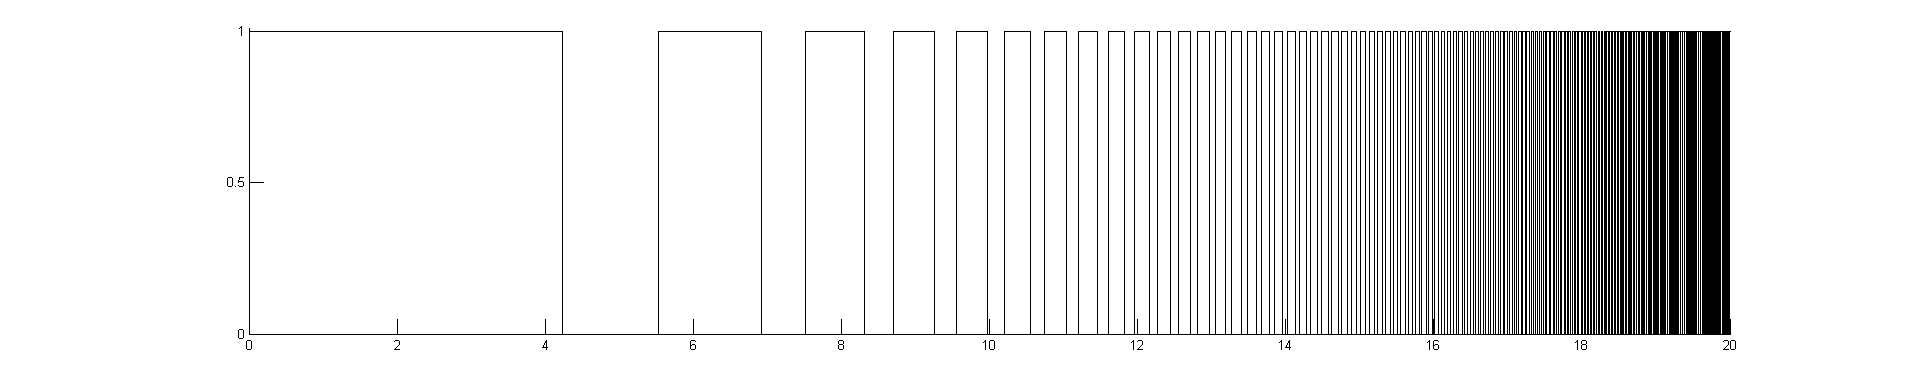
\includegraphics[width=120mm]{CW3-dwupolozeniowy-u-a0.png}
	\caption{Wykresy $\varepsilon(t)$, oraz $u(t)$ dla regulatora dwupoziomowego bez histerezy.}
    \label{fig:Rysunek}
\end{figure}

\newpage Widzimy z nich, że wykres błędu oscyluje z czasem coraz bliżej zera, więc wartość na wyjściu jest blisko pożądanej, lecz z czasem rośnie również częstotliwość przełączania regulatora, przez co znacznie rośnie jego zużycie i maleje żywotność.

\subsubsection{Regulator dwupołożeniowy z histerezą}\label{sec:r2h}%----------------------------------------------------------

%TODO-----------------------------------
%Opis działania histerezy
%Dokończyć rysunek (podpisać osie, etc)
%---------------------------------------

\begin{figure}[!h]
    \centering
	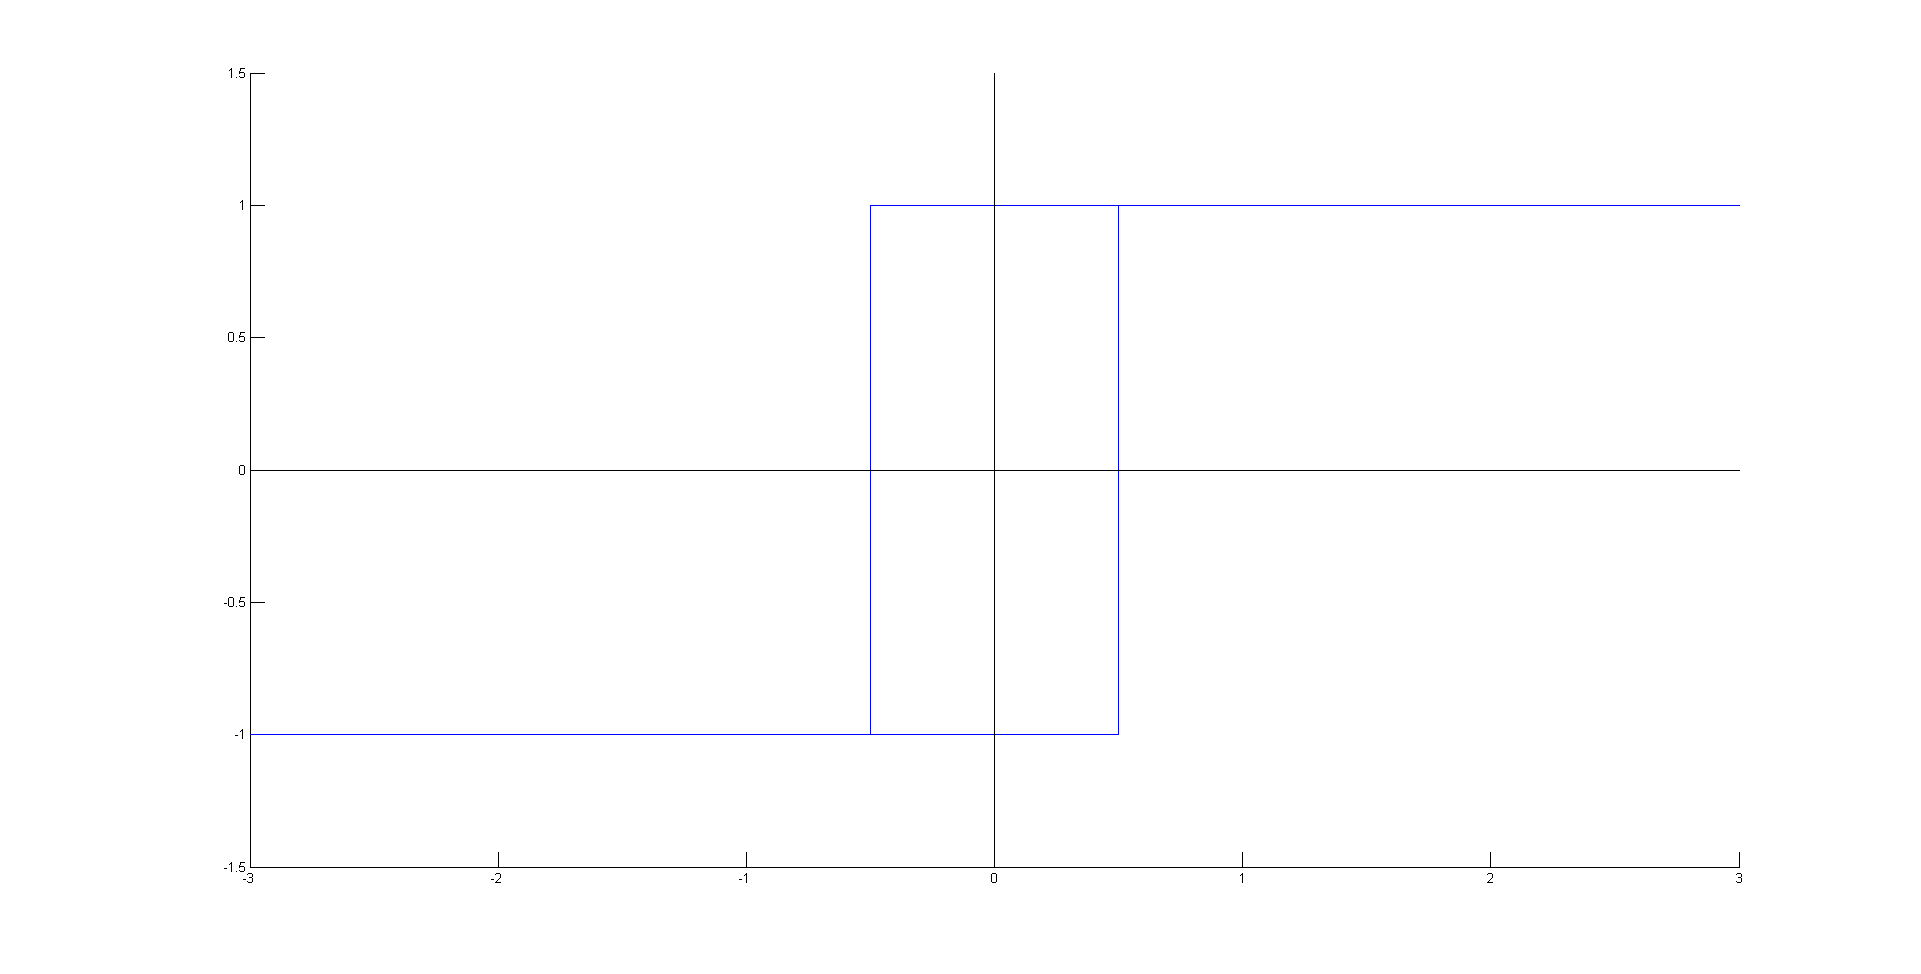
\includegraphics[width=120mm]{CW3-histereza-dwupoziomowa.png}
	\caption{Jak działa histereza dwupoziomowa.}
    \label{fig:Rysunek}
\end{figure}

Symulacje regulatora dwupoziomowego z histerezą przeprowadzimy na tym samym modelu, który posłużył nam w zadaniu \ref{sec:r2bh}, jednak w obiekcie 'Relay1' parametry 'On' i 'Off' będą różne, dzięki czemu ustawimy żądaną histerezę.\newpage
Za przeprowadzenie testu odpowiedzialna jest poniższa funkcja.

\begin{lstlisting}[caption=Funkcja testująca regulator dwupoziomowy z histerezą.]
function testDwupoziomowy2(step, stop, flag)
load_system('dwupoziomowy.mdl');
hold on;
i=1;
color = char('y', 'k', 'b', 'g', 'r', 'm');

while (step*i <= stop)
    set_param('dwupoziomowy/Relay1', 'On_switch_value', num2str(step*i));
    set_param('dwupoziomowy/Relay1', 'Off_switch_value', num2str(-step*i));

    sim('dwupoziomowy.mdl');
    figure(1);
    uwy= u.signals.values;    
    plot(tout, uwy, 'Color', color(mod(i,6)+1));

    figure(2);
    ewy= e.signals.values;    
    plot(tout, ewy, 'Color', color(mod(i,6)+1));

    if flag
        hold on;
        plot([0 30], [0 0], '-r');
        plot([0 30], [step*i step*i], strcat('--', color(mod(i,6)+1)));
        plot([0 30], [-step*i -step*i], strcat('--', color(mod(i,6)+1)));
    end

    i=i+1;
    hold all;
end
end
\end{lstlisting}

Po wywołaniu powyższej funkcji dla wartości (0.5, 0.6, true) otrzymaliśmy poniższe wykresy.

\begin{figure}[!h]
    \centering
	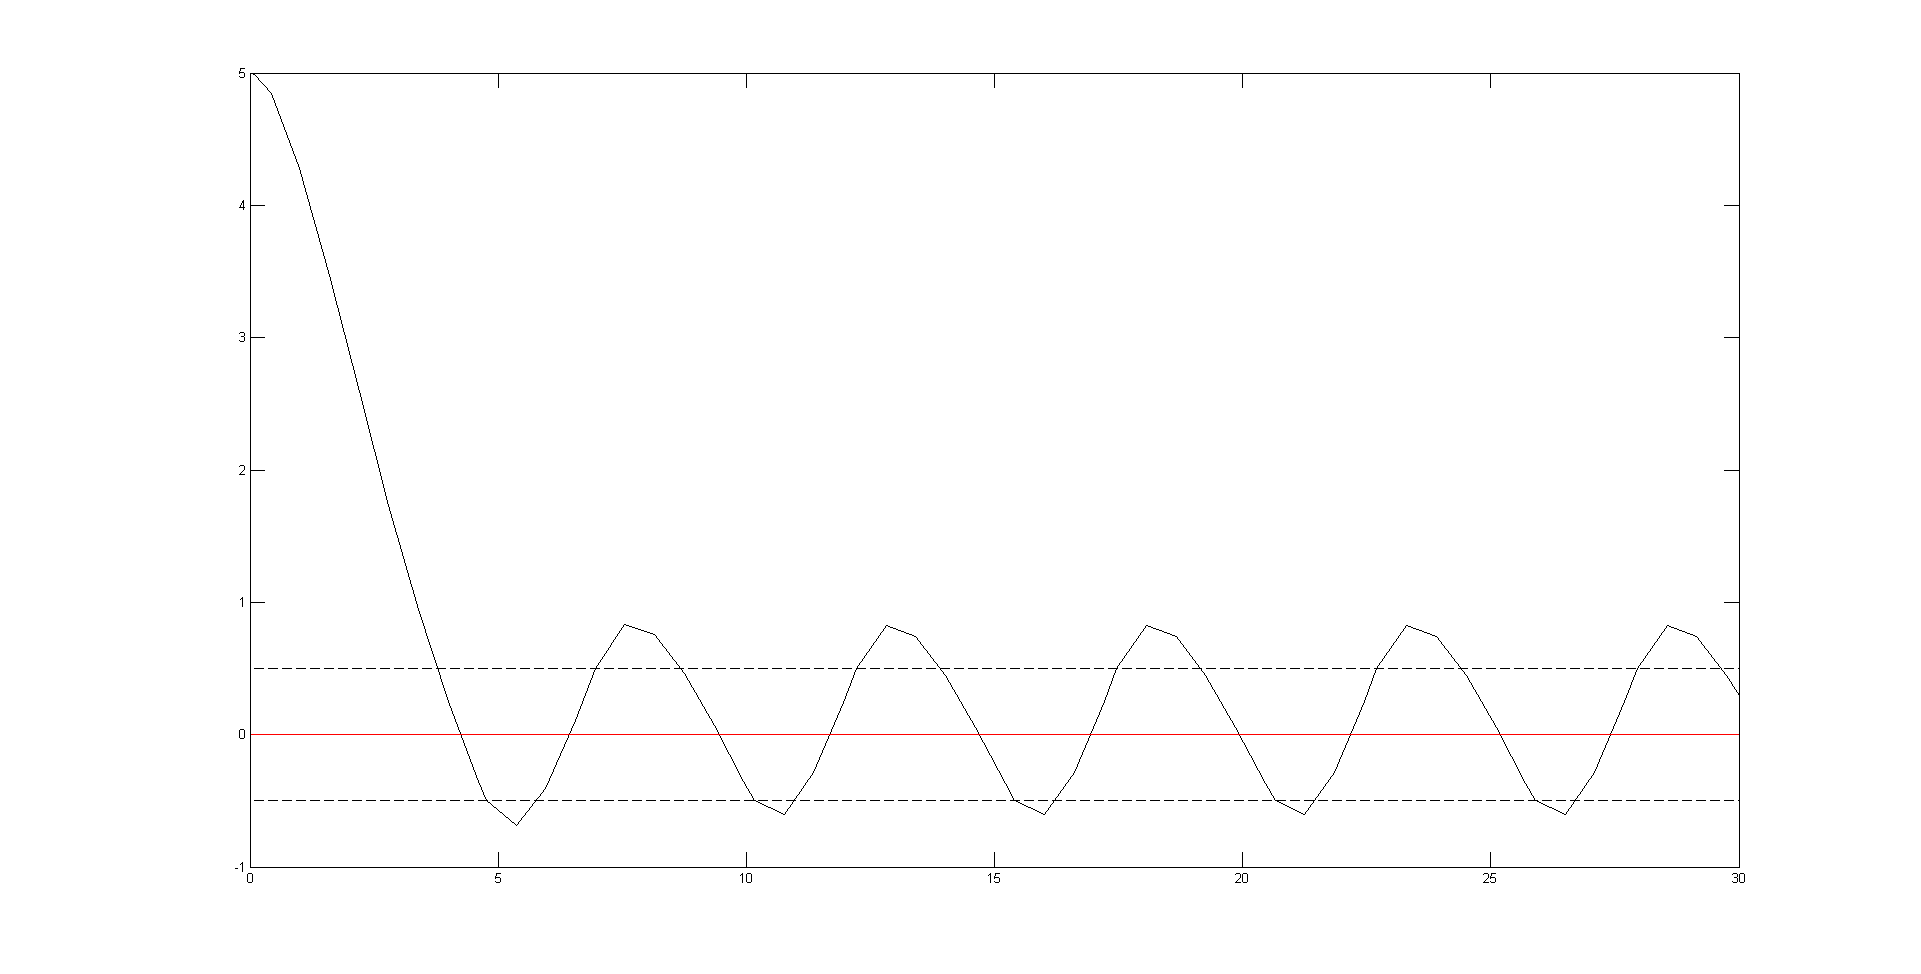
\includegraphics[width=120mm]{CW3-dwupolozeniowy-e-a05.png}
	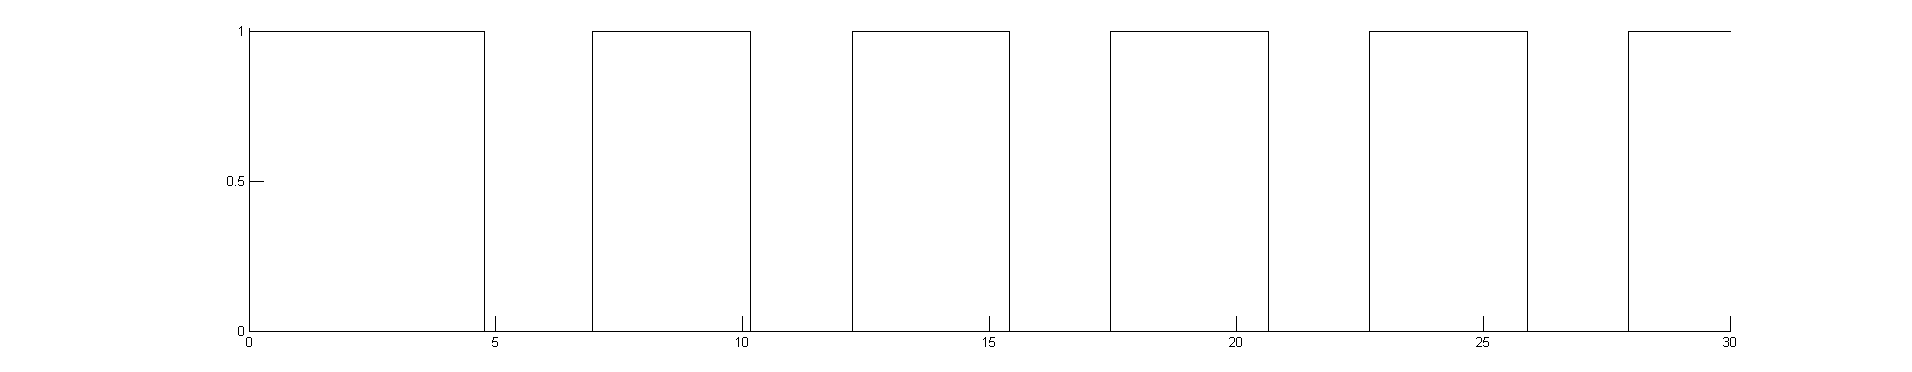
\includegraphics[width=120mm]{CW3-dwupolozeniowy-u-a05.png}
	\caption{Wykresy $\varepsilon(t)$, oraz $u(t)$ dla regulatora dwupoziomowego z histerezą.}
    \label{fig:Rysunek}
\end{figure}

Widzimy na nich, że amplituda oscylacji błędu wokół zera z czasem stabilizuje się, a liczba przełączeń znacznie maleje w stosunku do regulatora dwupoziomowego bez histerezy, a więc i wydłuża się jego żywotnosć. \\
Aby zbadać wpływ zakresu histerezy na wykres $\varepsilon(t)$ wywołamy funkcję dla wartości (0.5, 2, false), w wyniku czego otrzymamy poniższe wykresy.

\begin{figure}[!h]
    \centering
	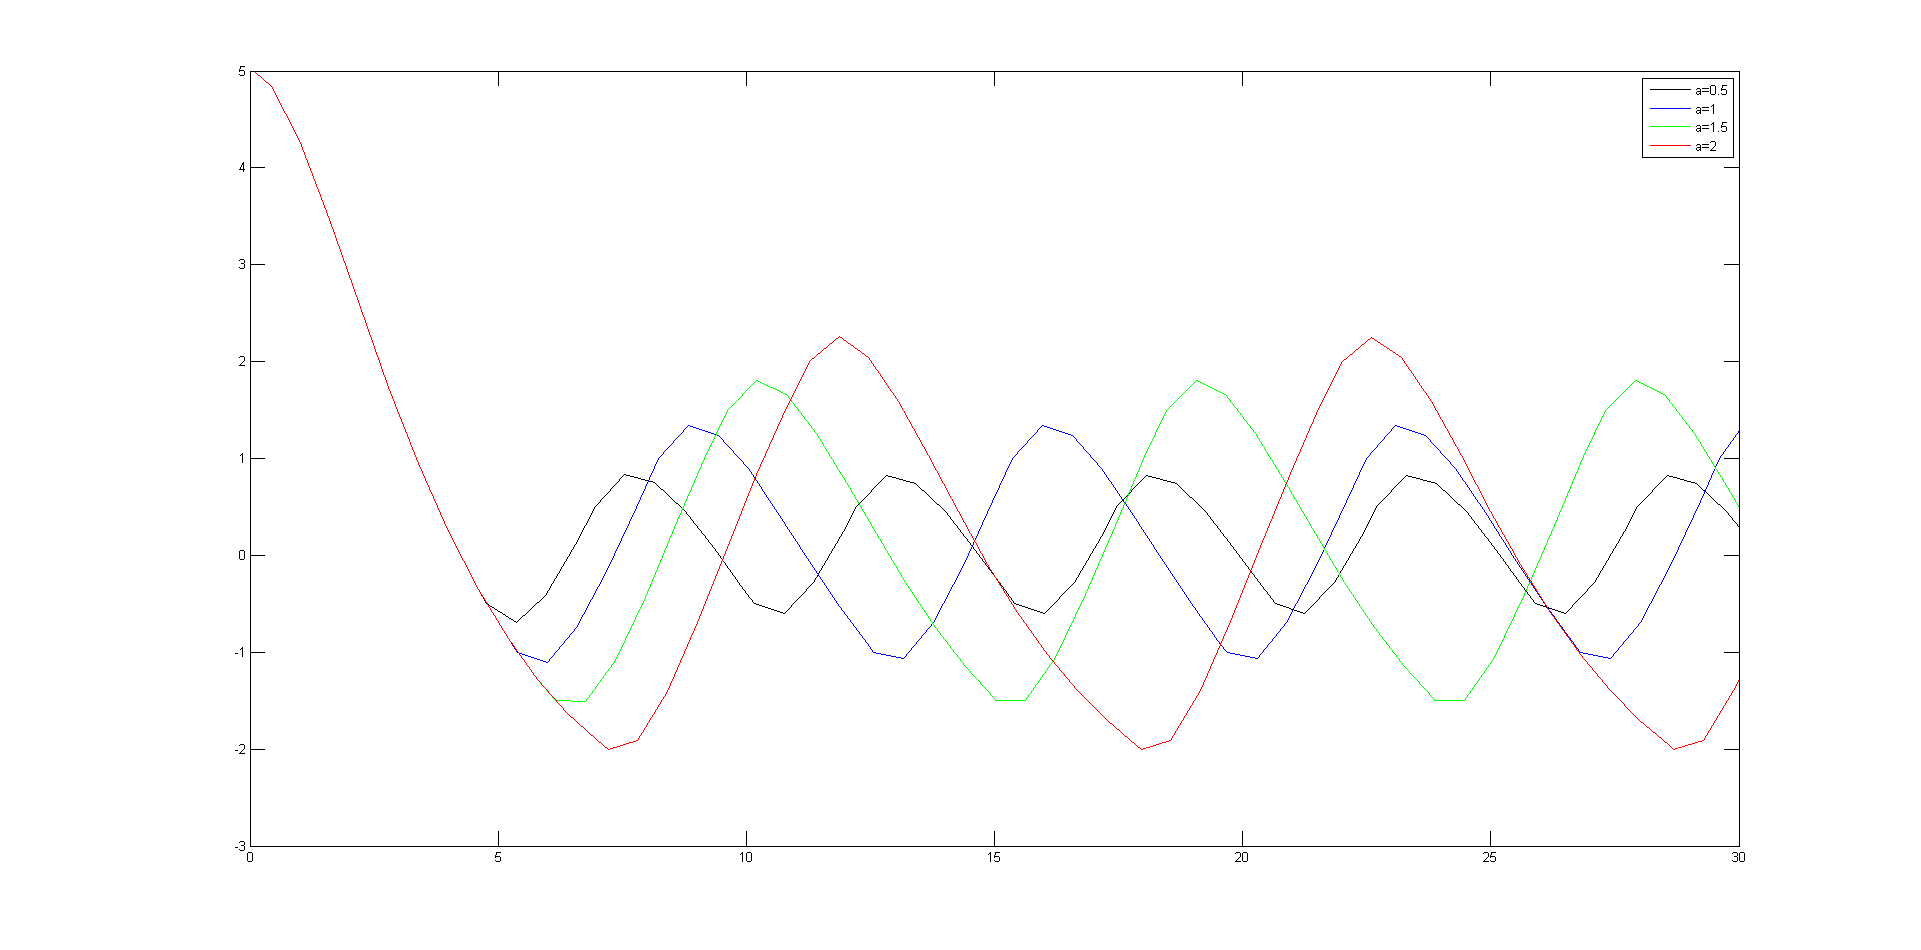
\includegraphics[width=120mm]{CW3-dwupolozeniowy-e.png}
	\caption{Pokazujemy jak się zmienia przy rosnącym $a$.}
    \label{fig:Rysunek}
\end{figure}

\newpage Widzimy na nich, że w miarę zwiększania zakresu histerezy rośnie amplituda oscylacji wykresu błędu wokół zera, oraz maleje częstotliwość przełączeń regulatora.

\subsubsection{Regulator trójpołożeniowy bez histerezy}\label{sec:r3bh}%----------------------------------------------------------

\begin{figure}[!h]
    \centering
	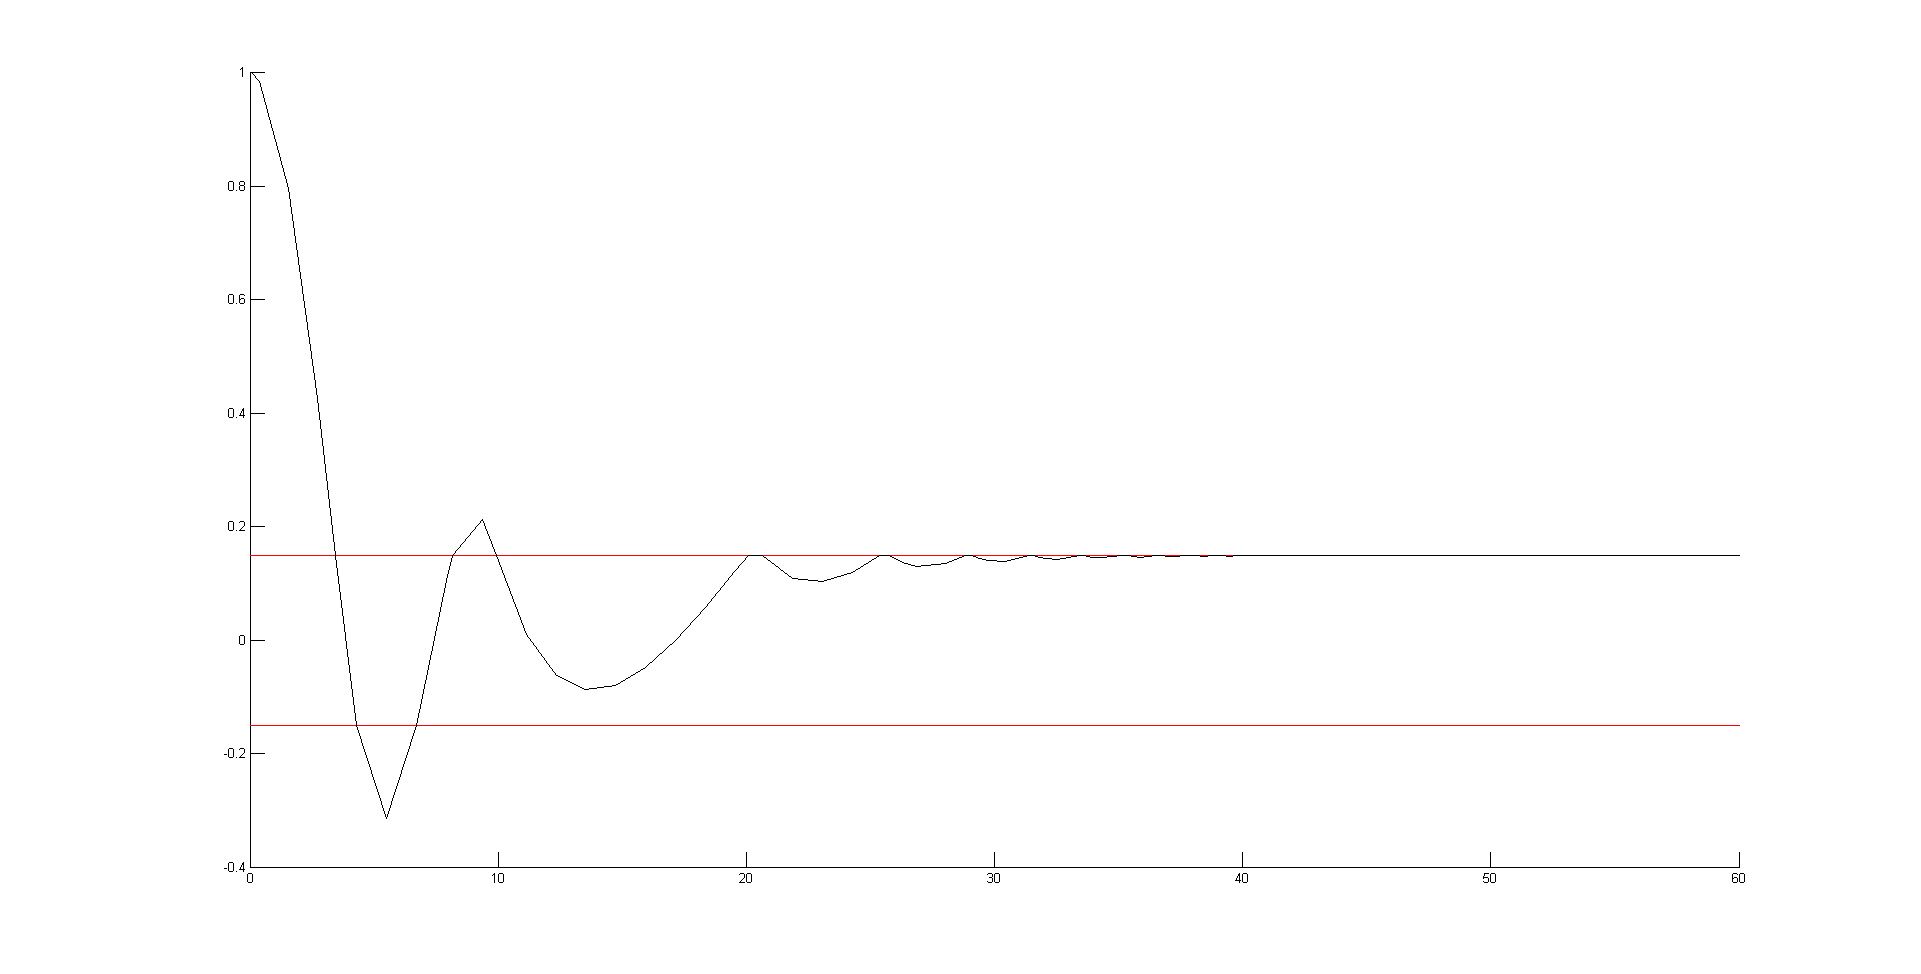
\includegraphics[width=120mm]{CW3-trojpolozeniowy-e-n015-a0.png}
	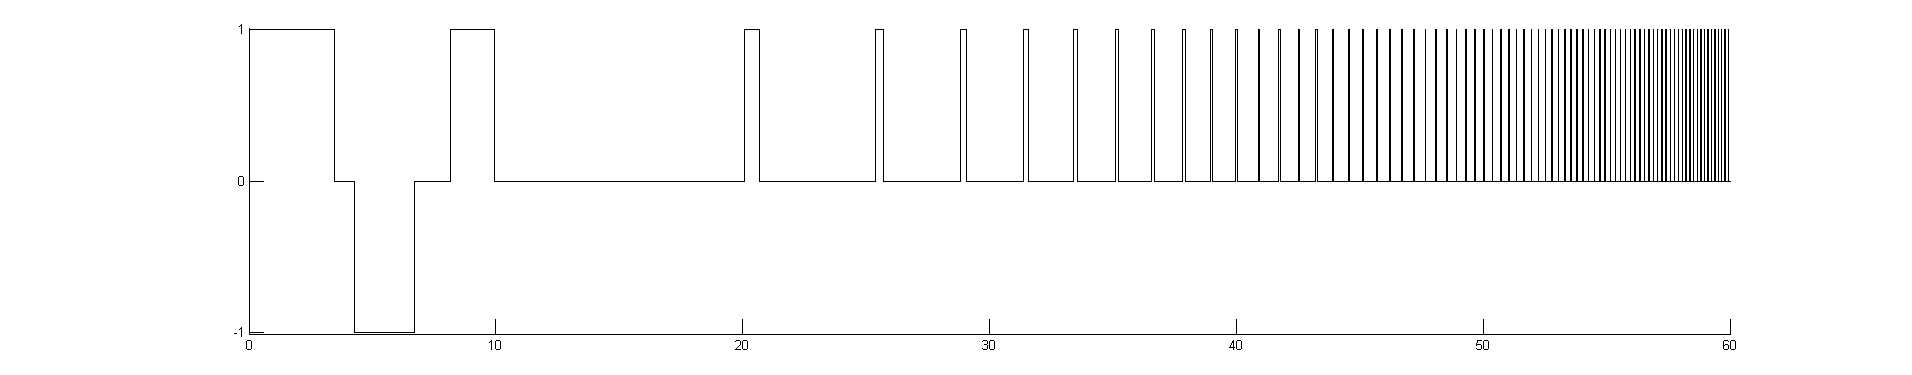
\includegraphics[width=120mm]{CW3-trojpolozeniowy-u-n015-a0.png}
	\caption{Pokazujemy kiedy się przełącza.}
    \label{fig:Rysunek}
\end{figure}

\subsubsection{Regulator trójpołożeniowy z histerezą}\label{sec:r3h}%----------------------------------------------------------

\begin{figure}[!h]
    \centering
	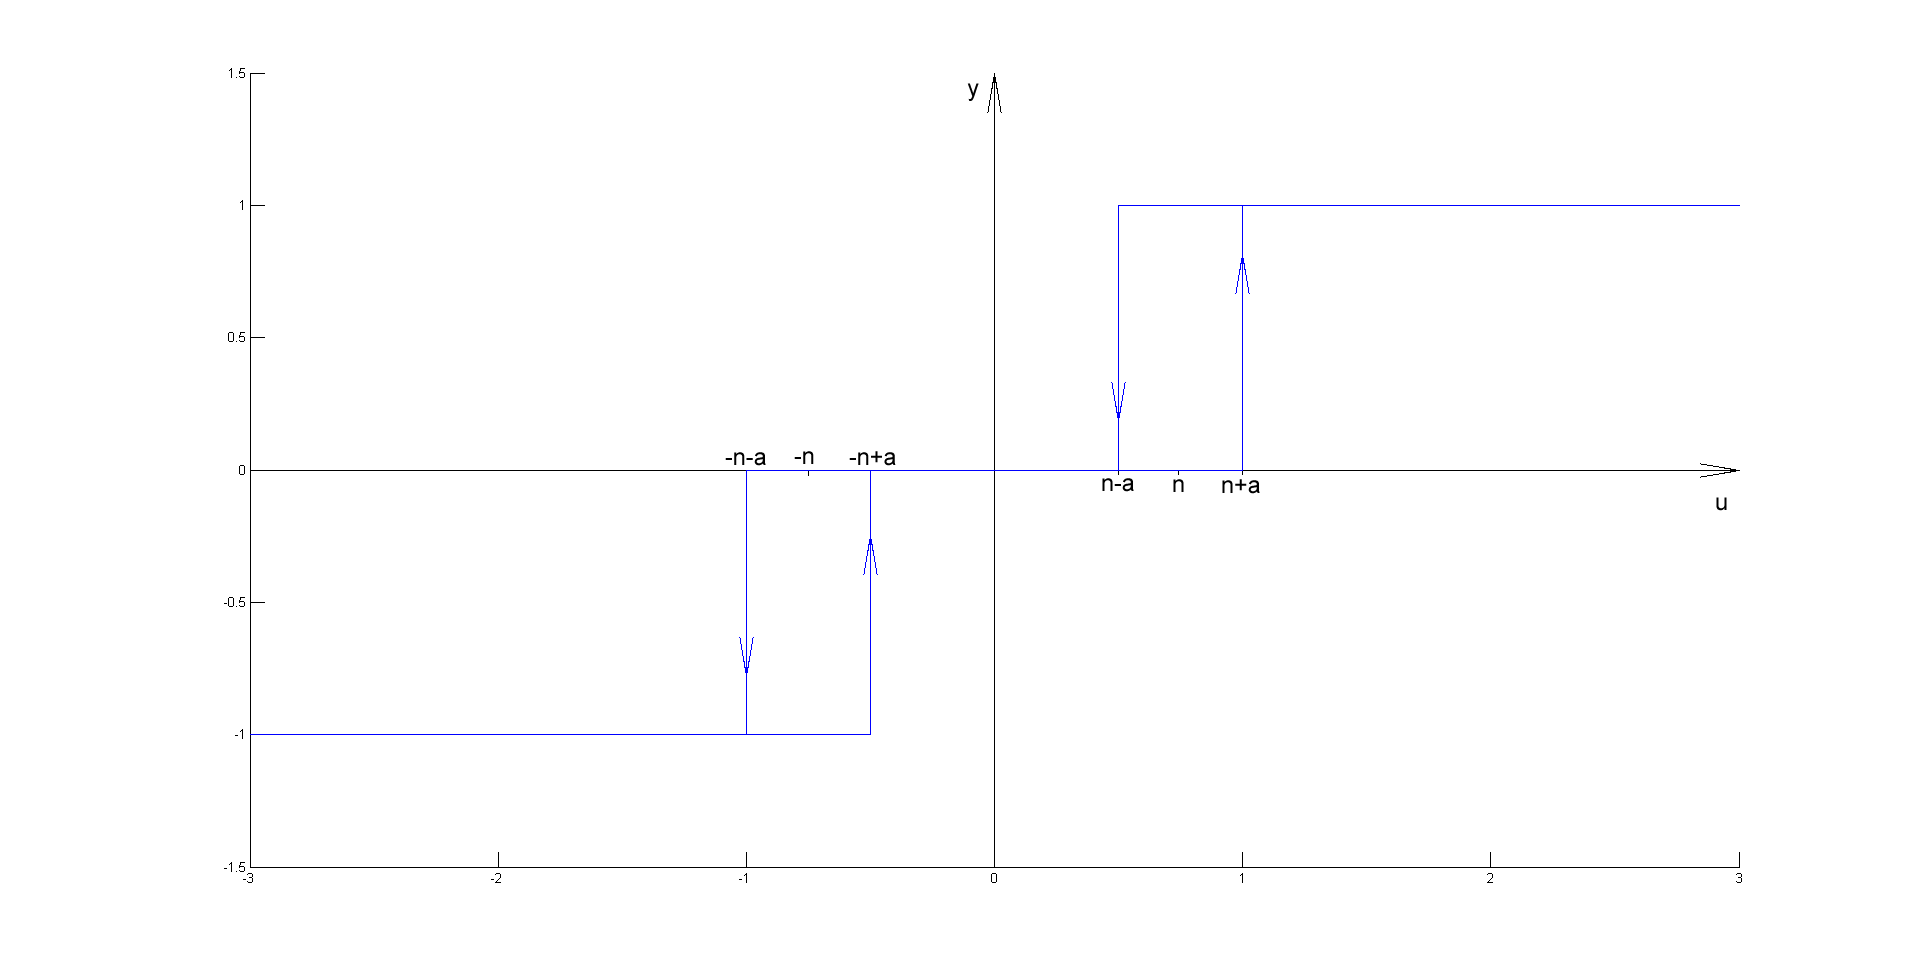
\includegraphics[width=120mm]{CW3-histereza-trojpoziomowa.png}
	\caption{Jak działa histereza trójpoziomowa.}
    \label{fig:Rysunek}
\end{figure}

\begin{figure}[!h]
    \centering
	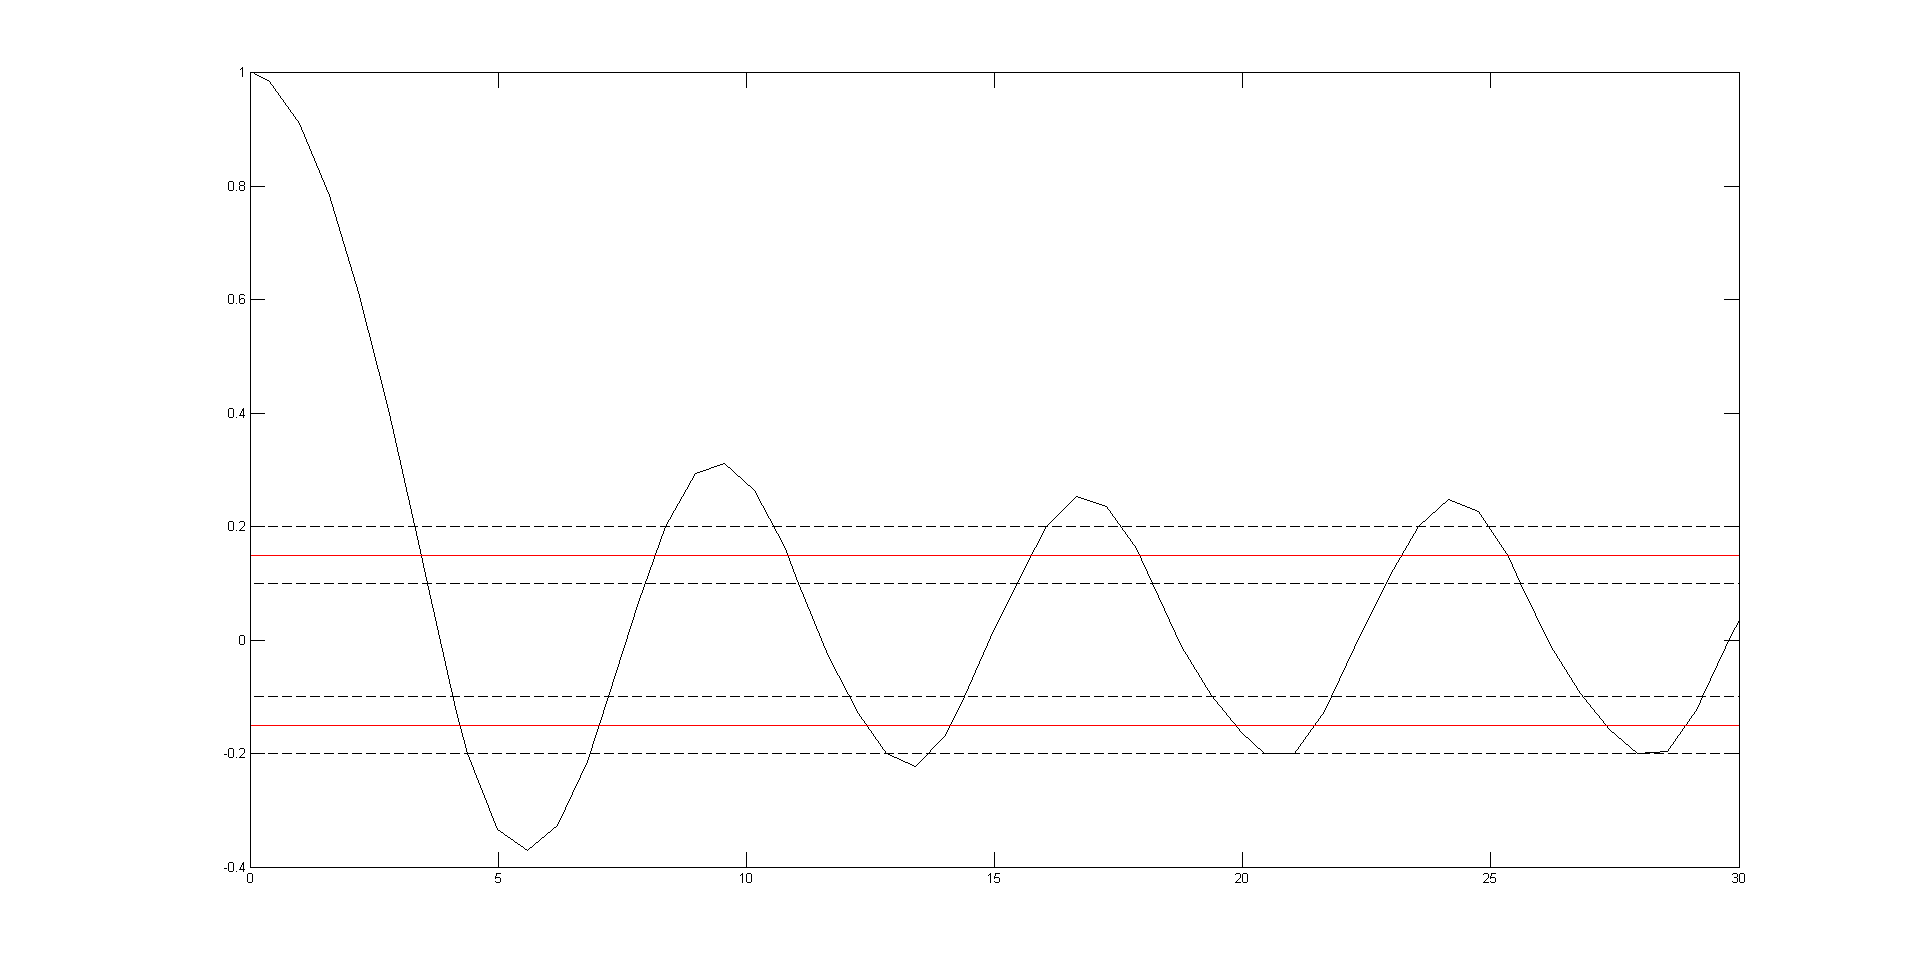
\includegraphics[width=120mm]{CW3-trojpolozeniowy-e-n015-a005.png}
	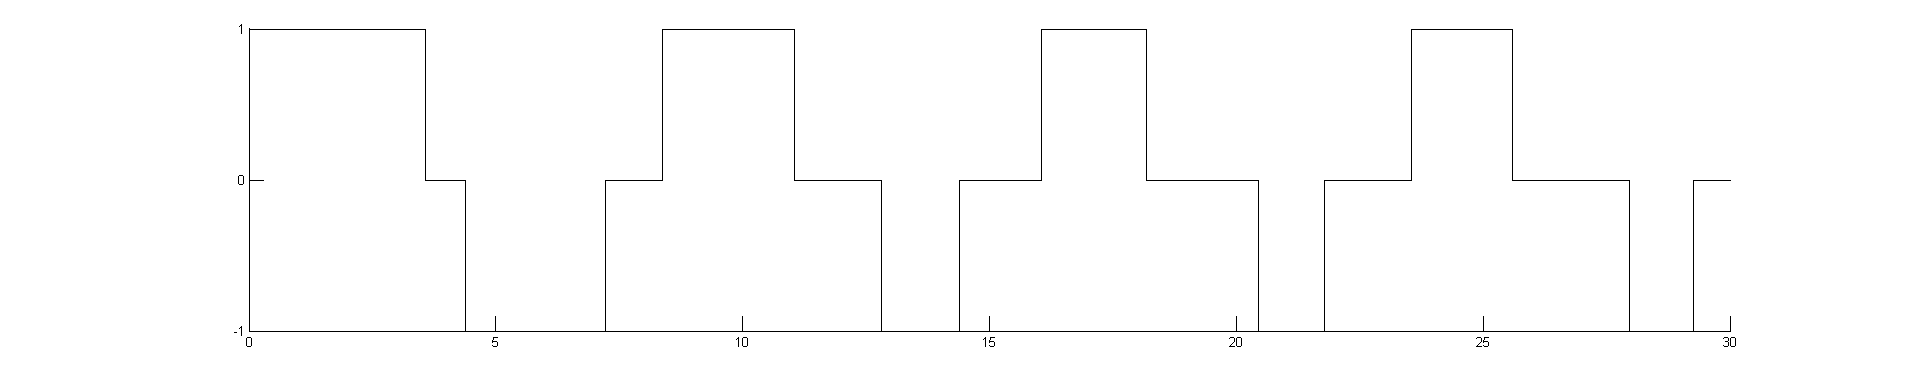
\includegraphics[width=120mm]{CW3-trojpolozeniowy-u-n015-a005.png}
	\caption{Pokazujemy kiedy się przełącza.}
    \label{fig:Rysunek}
\end{figure}

\begin{figure}[!h]
    \centering
	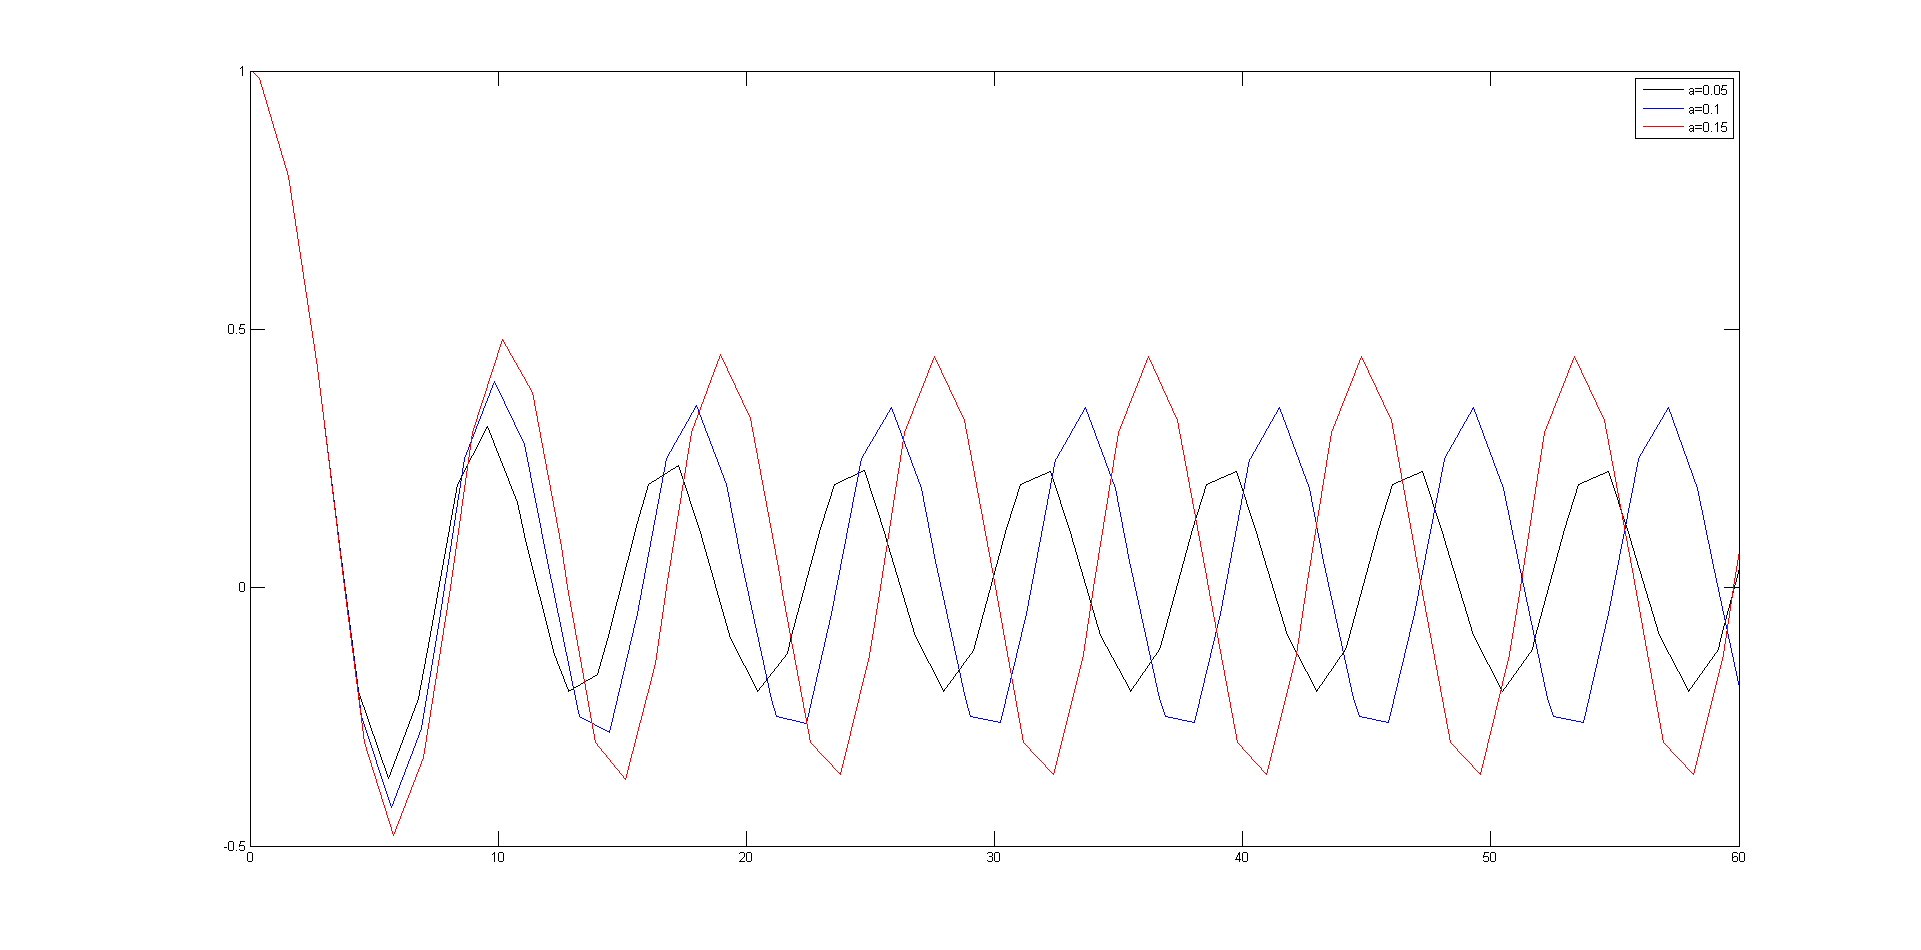
\includegraphics[width=120mm]{CW3-trojpolozeniowy-e-n015.png}
	\caption{Pokazujemy jak się zmienia przy rosnącym $a$.}
    \label{fig:Rysunek}
\end{figure}
%---------------------------------------------------------------------------------------------------------------------
%ZADANIE 2
%---------------------------------------------------------------------------------------------------------------------
\newpage
\subsection{Zastosowanie członów korekcyjnych.}\label{sec:zad2}
W tym zadaniu dodatkowo dodaliśmy człony korekcyjne, do poprzednich układów. Do układu została dodana również wartość stała.
\subsubsection{Modyfikacja systemów z zadania 1}\label{sec:zad2_1}
\begin{figure}[!h]
    \centering
	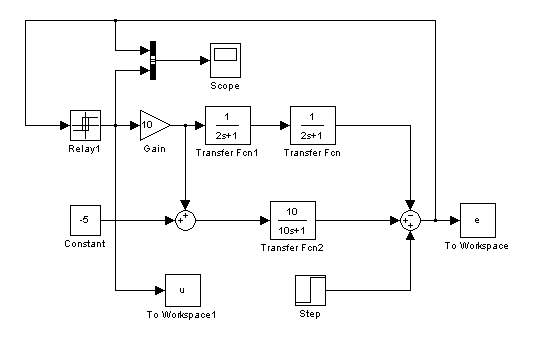
\includegraphics[width=120mm]{CW3-schemat-2k.png}
	\caption{fig:Schemat regulatora dwupolożeniowego z korekcją.}
    \label{fig:Rysunek}
\end{figure}
\begin{figure}[!h]
    \centering
	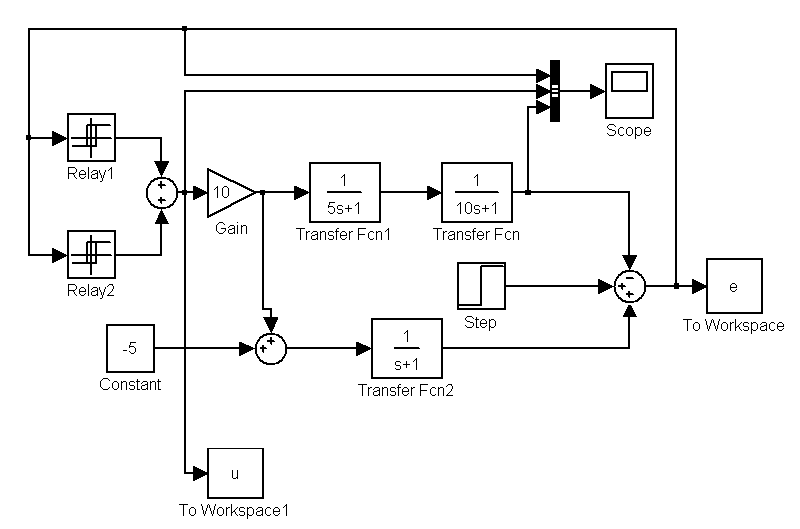
\includegraphics[width=120mm]{CW3-schemat-3k.png}
	\caption{fig:Schemat regulatora trojpolożeniowego z korekcją.}
    \label{fig:Rysunek}
\end{figure}
\subsubsection{Doświadczalny dobor parametrów członu korekcyjnego.}\label{sec:zad2_2}
\begin{enumerate}
		\item Regulator dwupołożeniowy.
		
\begin{lstlisting}[caption=Funkcja testująca regulator dwupoziomowy z korekcją zmiana T.]
function testDwupoziomowyKorekcjaT(start,step, stop)
load_system('dwupoziomowyKorekcja.mdl');
hold on;
i=1;
color = char('y', 'k', 'b', 'g', 'r', 'm');
legendtext{1}='';
legendtext1{1}='';
while (start+step*i <= stop)
        set_param('dwupoziomowyKorekcja/Transfer Fcn2', 'Denominator', strcat('[',num2str(start+step*i),' 1]'));
        sim('dwupoziomowyKorekcja.mdl');
        figure(1);
        uwy= u.signals.values;    
        plot(tout, uwy, 'Color', color(mod(i,6)+1));        
        legendtext{i}= strcat('Tk=' , num2str(start+step*i));
        legend(legendtext1);
        figure(2);
        ewy= e.signals.values;    
        plot(tout, ewy, 'Color', color(mod(i,6)+1));        
        legendtext1{i}= strcat('Tk=' , num2str(start+step*i));
        legend(legendtext1);
        i=i+1;
        hold all;
end
end
\end{lstlisting}
Analogicznie do testowania K i C
\begin{lstlisting}[caption=set param dla K.]
set_param('dwupoziomowyKorekcja/Transfer Fcn2', 'Numerator', num2str(start+step*i));
\end{lstlisting}
\begin{lstlisting}[caption=set param dla C.]
set_param('dwupoziomowyKorekcja/Constant', 'value', num2str(start+step*i));
\end{lstlisting}

Dla układu z histerezą, otrzymaliśmy następujące wykresy:
\begin{figure}[!h]
    \centering
	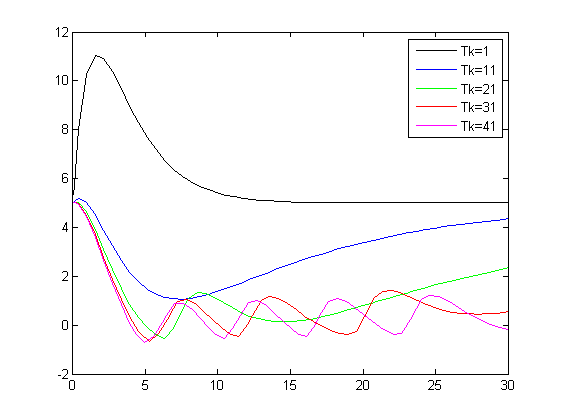
\includegraphics[width=120mm]{CW3-korekcja-dwupolozeniowy-e_Tk.png}
	\caption{Zmiana Tk przy stałym k=1 i C=0}
    \label{fig:Rysunek}
\end{figure}
\begin{figure}[!h]
    \centering
	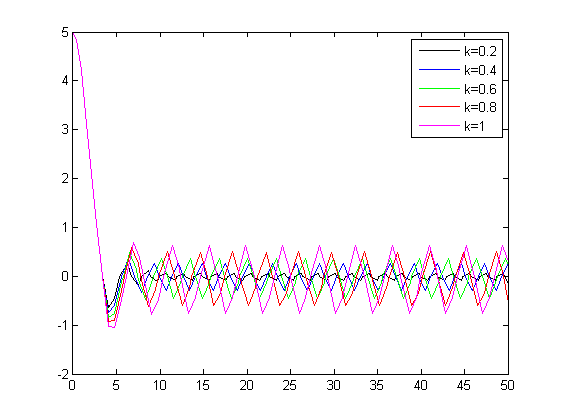
\includegraphics[width=120mm]{CW3-korekcja-dwupolozeniowy-e_k.png}
	\caption{Zmiana k przy stałym Tk=1 i C=0}
    \label{fig:Rysunek}
\end{figure}
\begin{figure}[!h]
    \centering
	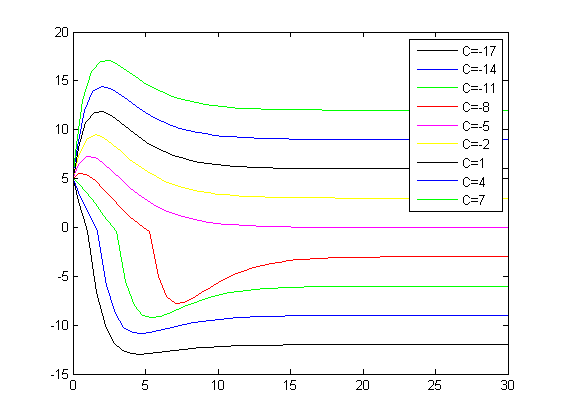
\includegraphics[width=120mm]{CW3-korekcja-dwupolozeniowy-e_C_k1T1.png}
	\caption{Zmiana C przy stałym k=1 i Tk=1}
    \label{fig:Rysunek}
\end{figure}

Widać, że układ najlepiej zachoduje się gdy Kk=1 i T=1.

Dla układu bez histerezy otrzymaliśmy bardzo podobne wyniki:
\begin{figure}[!h]
    \centering
	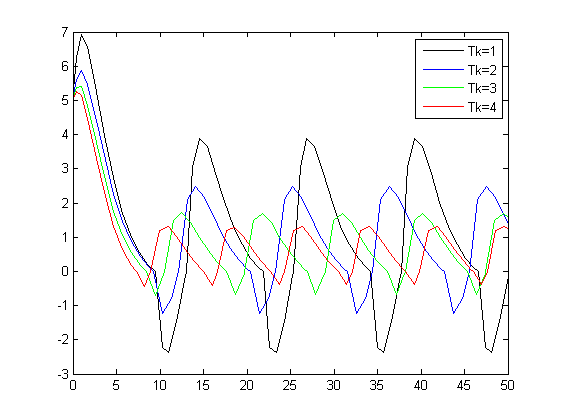
\includegraphics[width=120mm]{CW3-korekcja-dwupolozeniowyBH-e_Tk.png}
	\caption{Zmiana Tk przy stałym k=1 i C=0}
    \label{fig:Rysunek}
\end{figure}

\begin{figure}[!h]
    \centering
	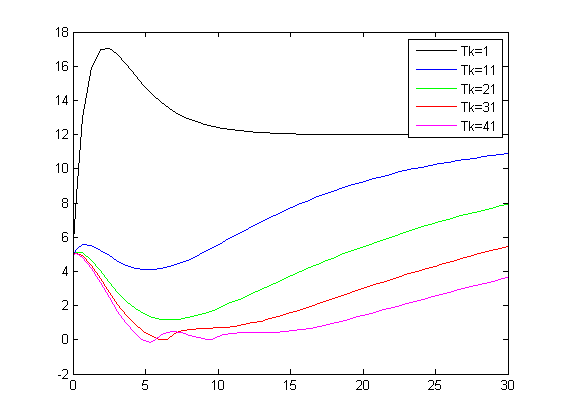
\includegraphics[width=120mm]{CW3-korekcja-dwupolozeniowyBH-e_k.png}
	\caption{Zmiana k przy stałym Tk=1 i C=0}
    \label{fig:Rysunek}
\end{figure}

\begin{figure}[!h]
    \centering
	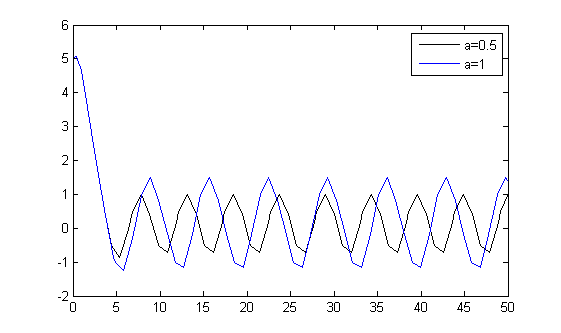
\includegraphics[width=120mm]{CW3-korekcja-dwupolozeniowy-e_a.png}
	\caption{Przy zmianie a}
    \label{fig:Rysunek}
\end{figure}



		\item Regulator trójpołożeniowy
		
\begin{figure}[!h]
    \centering
	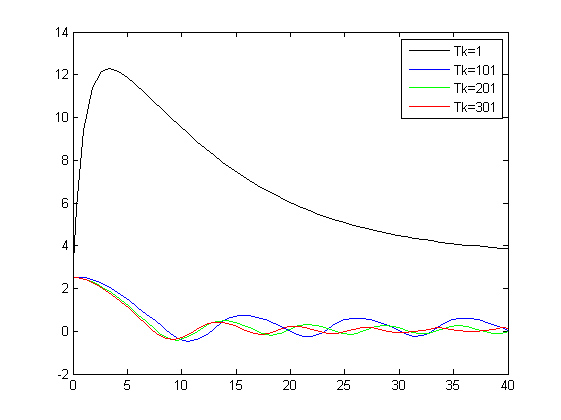
\includegraphics[width=120mm]{CW3-korekcja-trojpolozeniowy-e_Tk.png}
	\caption{Przy zmianie a}
    \label{fig:Rysunek}
\end{figure}

\begin{figure}[!h]
    \centering
	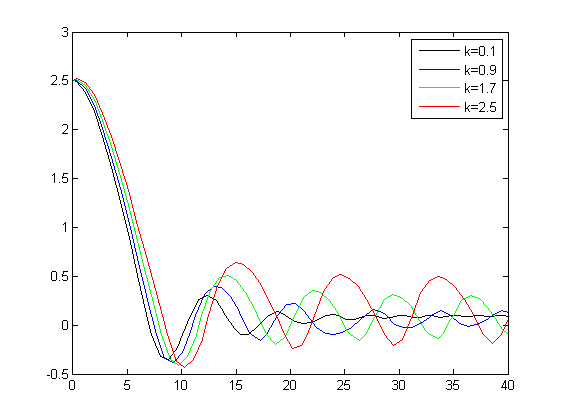
\includegraphics[width=120mm]{CW3-korekcja-trojpolozeniowy-e_k.png}
	\caption{Przy zmianie a}
    \label{fig:Rysunek}
\end{figure}

\begin{figure}[!h]
    \centering
	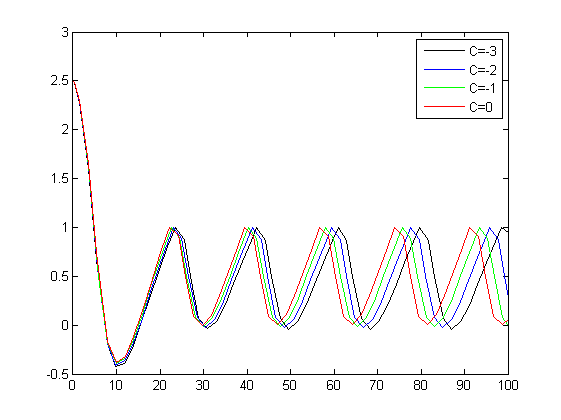
\includegraphics[width=120mm]{CW3-korekcja-trojpolozeniowy-e_C.png}
	\caption{Przy zmianie a}
    \label{fig:Rysunek}
\end{figure}

Stała nie wpływa na wynik.

\begin{figure}[!h]
    \centering
	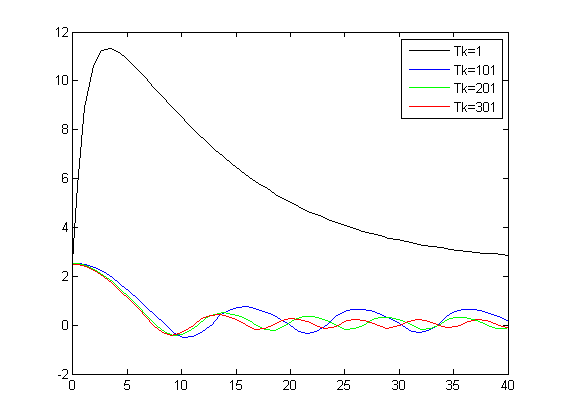
\includegraphics[width=120mm]{CW3-korekcja-trojpolozeniowyBH-e_Tk.png}
	\caption{Przy zmianie a}
    \label{fig:Rysunek}
\end{figure}

\begin{figure}[!h]
    \centering
	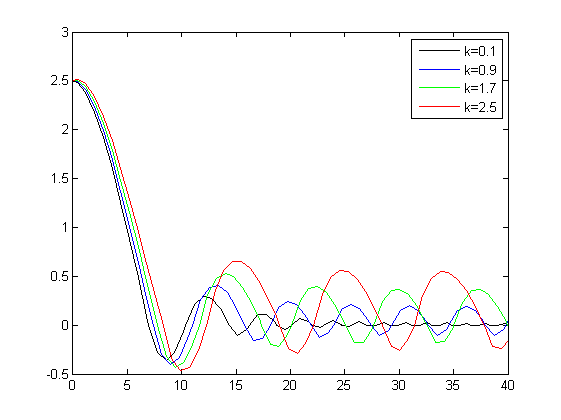
\includegraphics[width=120mm]{CW3-korekcja-trojpolozeniowyBH-e_k.png}
	\caption{Przy zmianie a}
    \label{fig:Rysunek}
\end{figure}

\end{enumerate}

\section{Wnioski.}\label{sec:wnioski}
TODO!!
\end{document}